\subsection{UC 15 - Modifica condivisione di una cartella} \label{sec:UC15}

    \begin{itemize}
        \item \textbf{Attore principale}: MUA;
        \item \textbf{Descrizione}: il MUA deve poter modificare una condivisione di una cartella nel sistema;
        \item \textbf{Precondizioni}: il MUA sta usando la funzionalità di modifica di una condivisione;
        \item \textbf{Postcondizioni}: il sistema modifica la condivisione della cartella con le informazioni fornite dal MUA;
        \item \textbf{Scenario principale}:
            \begin{enumerate}
                \item il MUA trasmette l'id della cartella condivisa (\hyperref[sec:UC15.1]{UC 15.1});
                \item il MUA trasmette il nuovo indirizzo e-mail a cui condividere (\hyperref[sec:UC15.2]{UC 15.2});
                \item il sistema condivide la cartella;
            \end{enumerate}
        \item \textbf{Inclusioni}: nessuna;
        \item \textbf{Generalizzazioni}: nessuna;
        \item \textbf{Estensioni}: nessuna.
    \end{itemize}

    \begin{figure}[H]
        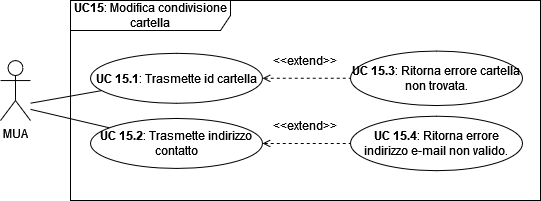
\includegraphics[width=0.85\textwidth]{sections/uc_imgs/UC15.png}
        \centering
        \caption{Diagramma sotto-casi UC 15}
    \end{figure}

    \subsubsection{UC 15.1 - Trasmette id cartella} \label{sec:UC15.1}
    \begin{itemize}
        \item \textbf{Attore principale}: MUA;
        \item \textbf{Descrizione}: il MUA trasmette l'id della cartella per modificare la condivisione della cartella;
        \item \textbf{Precondizioni}: il MUA sta usando la funzionalità di modifica condivisione di una cartella;
        \item \textbf{Postcondizioni}: il sistema conosce l'id della cartella di cui modificare la condivisione;
        \item \textbf{Scenario principale}:
            \begin{enumerate}
                \item il MUA invia l'id della cartella per modificare la condivisione della cartella;
            \end{enumerate}
        \item \textbf{Inclusioni}: nessuna;
        \item \textbf{Generalizzazioni}: nessuna;
        \item \textbf{Estensioni}:
            \begin{enumerate}[label=\alph*.]
                \item il sistema non riesce a modificare la condivisione della cartella perché l'id della cartella fornito non è stato trovato:
                \begin{enumerate}[label=\arabic*.]
                    \item il sistema ritorna un errore al MUA di cartella non trovata (\hyperref[sec:UC4.3]{UC 4.3}).
                \end{enumerate}
            \end{enumerate}
    \end{itemize}


    \subsubsection{UC 15.2 - Trasmette indirizzo e-mail} \label{sec:UC15.2}
    \begin{itemize}
        \item \textbf{Attore principale}: MUA;
        \item \textbf{Descrizione}: il MUA trasmette il nuovo indirizzo e-mail per la condivisione al sistema;
        \item \textbf{Precondizioni}: il MUA sta usando la funzionalità di modifica condivisione di una cartella;
        \item \textbf{Postcondizioni}: il sistema conosce il nuovo indirizzo e-mail a cui condividere;
        \item \textbf{Scenario principale}:
            \begin{enumerate}
                \item il MUA invia il nuovo indirizzo e-mail la condivisione al sistema;
                \item il sistema controlla che le informazioni ricevute rispettino il seguente requisito minimo:
                    \begin{itemize}
                        \item l'indirizzo email del contatto non è una stringa vuota;
                    \end{itemize}
            \end{enumerate}
        \item \textbf{Inclusioni}: nessuna;
        \item \textbf{Generalizzazioni}: nessuna;
        \item \textbf{Estensioni}:
            \begin{enumerate}[label=\alph*.]
                \item il sistema non riesce a creare il contatto perché l'indirizzo e-mail fornito non è valido:
                \begin{enumerate}[label=\arabic*.]
                    \item il sistema ritorna un errore al MUA di indirizzo e-mail non valido (\hyperref[sec:UC15.4]{UC 15.4}).
                \end{enumerate}
            \end{enumerate}
    \end{itemize}


\subsubsection{UC 15.3 - Ritorna errore cartella non trovata} \label{sec:UC15.3}
    \begin{itemize}
        \item \textbf{Attore principale}: MUA;
        \item \textbf{Descrizione}: il sistema non riesce a modificare la condivisione della cartella perché la cartella non è stata trovata;
        \item \textbf{Precondizioni}: il MUA ha inviato l'id della cartella da condividere;
        \item \textbf{Postcondizioni}: il sistema non modifica la condivisione della cartella, il MUA è stato notificato dell'errore;
        \item \textbf{Scenario principale}:
            \begin{enumerate}
                \item il sistema non trova la cartella con l'identificativo fornito dal MUA;
                \item il sistema non modifica la condivisione della cartella e notifica il MUA dell'errore;
            \end{enumerate}
        \item \textbf{Inclusioni}: nessuna;
        \item \textbf{Generalizzazioni}: nessuna;
        \item \textbf{Estensioni}: nessuna.
    \end{itemize}

    \subsubsection{UC 15.4 - Ritorna errore indirizzo e-mail non valido} \label{sec:UC15.4}
    \begin{itemize}
        \item \textbf{Attore principale}: MUA;
        \item \textbf{Descrizione}: il sistema non riesce a modificare la condivisione della cartella perché l'indirizzo e-mail del contatto non rispetta i requisiti;
        \item \textbf{Precondizioni}: il MUA ha inviato il nuovo indirizzo e-mail a cui condividere;
        \item \textbf{Postcondizioni}: il sistema non modifica la condivisione della cartella, il MUA è stato notificato dell'errore;
        \item \textbf{Scenario principale}:
            \begin{enumerate}
                \item il sistema controlla la sintassi dell'indirizzo e-mail e trova un errore;
                \item il sistema non modifica la condivisione della cartella e notifica il MUA dell'errore;
            \end{enumerate}
        \item \textbf{Inclusioni}: nessuna;
        \item \textbf{Generalizzazioni}: nessuna;
        \item \textbf{Estensioni}: nessuna.
    \end{itemize}
